\documentclass[conference]{IEEEtran}
\IEEEoverridecommandlockouts

% Standard IEEE conference packages
\usepackage{cite}
\usepackage{amsmath,amssymb,amsfonts}
\usepackage{algorithmic}
\usepackage{graphicx}
\usepackage{textcomp}
\usepackage{xcolor}
\usepackage{booktabs}
\usepackage{tabularx}
\usepackage{url}
\usepackage{hyperref}
\usepackage{microtype}
\usepackage{subcaption}
\usepackage{tikz}
\usetikzlibrary{shapes.geometric, arrows.meta, positioning, fit, backgrounds, calc}

\hypersetup{
    colorlinks=true,
    linkcolor=black,
    citecolor=black,
    urlcolor=blue
}


% Spacing adjustments for strict 6-page IEEE conference budget
\setlength{\textfloatsep}{7pt plus 1.5pt minus 1.5pt}
\setlength{\floatsep}{6pt plus 1.5pt minus 1.5pt}
\setlength{\intextsep}{6pt plus 1.5pt minus 1.5pt}
\setlength{\dbltextfloatsep}{7pt plus 1.5pt minus 1.5pt}
\setlength{\dblfloatsep}{6pt plus 1.5pt minus 1.5pt}
\setlength{\abovedisplayskip}{3.5pt plus 1pt minus 1pt}
\setlength{\belowdisplayskip}{3.5pt plus 1pt minus 1pt}
\setlength{\abovedisplayshortskip}{2pt plus 1pt minus 0.5pt}
\setlength{\belowdisplayshortskip}{2pt plus 1pt minus 0.5pt}
\begin{document}

\title{Uncertainty-Aware 3D Vision-Language and Motion Mapping from Consumer Mobile LiDAR Scans\\
\thanks{This research was prepared for submission to the IEEE International Conference on Modelling, Simulation and Intelligent Computing (MoSICom 2026) at BITS Pilani, Dubai Campus.}
}

\author{\IEEEauthorblockN{Research Author\textsuperscript{1}, Advising Faculty\textsuperscript{1}}
\IEEEauthorblockA{\textit{\textsuperscript{1}Department of Computer Science and Engineering} \\
\textit{Academic Institution / University}\\
City, Country \\
Emails: \{author, faculty\}@institution.edu}
}

\maketitle

\begin{abstract}
Open-vocabulary 3D scene mapping enables autonomous robots and spatial AI systems to ground natural-language queries in physical space. While recent frameworks such as Visual Language Maps (VLMaps) and Vision-Language-Motion Maps (VLMM) address static and dynamic spatial reasoning, existing formulations assume research-grade RGB-D sensors providing pre-calibrated floating-point metric depth. When deployed on handheld consumer devices---such as Apple iPhone LiDAR streams recorded via Record3D---these systems encounter severe real-world degradation: 8-bit normalized depth quantization without confidence masks, camera coordinate-system discrepancies, high-frequency handheld camera shake, and persistent detector hallucinations that corrupt 3D spatial memory. In this paper, we present an uncertainty-aware 3D vision-language and motion mapping framework specifically adapted for lossy consumer mobile LiDAR recordings. Our methodology introduces three core contributions: (1) A multi-view epipolar calibration and temporally regularized affine depth decoder that reduces median epipolar residual error from 20.81~px to 0.298~px and median absolute relative depth error from 31.53\% to 3.76\%; (2) An open-vocabulary semantic verification gate with margin-based abstention using CLIP ViT-B/32, correcting 86.7\% (13 of 15) of persistent detector misidentifications from YOLO11n; and (3) An adaptation of VLMM's geometric motion-residual formulation that couples persistent Segment Anything Model (SAM~3.1) video-tracked masks with consumer depth-decoder uncertainty propagation. Our adaptation achieves a 23.8\% gain in valid motion pixel correspondences (from 7,529 to 9,322 pixels) over bounding-box baselines and a 4.5\% gain over single-frame SAM~3 spatial masks, while suppressing static background parallax bleed under handheld camera jitter. Finally, Screened Poisson surface reconstruction is integrated as a supporting geometry-completion method, generating watertight 3D meshes (216,243 vertices, 446,214 triangles) from occluded mobile point clouds.
\end{abstract}

\begin{IEEEkeywords}
3D Scene Reconstruction, Mobile LiDAR, Vision-Language Maps, VLMM Adaptation, SAM 3, SAM 3.1, Semantic Verification, Motion Modeling.
\end{IEEEkeywords}

\section{Introduction}
Spatial AI and mobile robotics increasingly rely on open-vocabulary 3D scene maps that ground unconstrained natural-language queries in physical space~\cite{radford2021clip, huang2023vlmaps, jatavallabhula2023conceptfusion}. To advance beyond static representations, Ghosh and Shakya recently introduced Vision-Language-Motion Maps (VLMM)~\cite{vlmm2026}, proposing a dual-channel architecture that combines VLM-derived semantic movability priors with geometric cross-frame motion observations and per-element uncertainty modeling.

However, a substantial gap separates existing open-vocabulary mapping frameworks from commodity mobile hardware. Prior systems are typically evaluated on benchmark datasets (e.g., ScanNet, Replica, or synthetic simulations) that supply calibrated floating-point metric depth, factory-calibrated camera matrices, and controlled robotic trajectories. In contrast, commodity consumer smartphones---specifically Apple iPhone Pro devices equipped with direct Time-of-Flight (dToF) LiDAR sensors and ARKit 6-DoF tracking, recorded via utilities like Record3D~\cite{apple2020arkit}---export data subject to severe real-world constraints:
\begin{enumerate}\setlength{\itemsep}{1.5pt}\setlength{\parskip}{0pt}
    \item \textbf{Lossy Depth and Coordinate Inconsistencies:} Mobile capture utilities frequently compress raw floating-point LiDAR depth into normalized 8-bit integer arrays ($0$--$255$) to conserve storage and bandwidth, omitting native per-pixel confidence masks, focal lengths, and display-orientation transformations. Directly projecting these raw exports causes severe 3D warping, wall shearing, and dimensional collapse.
    \item \textbf{Semantic Hallucination Accumulation:} Standard 2D object detectors exhibit persistent category confusion across sequential frames (e.g., consistently classifying an orange beanbag chair as a ``bed''). In naive multi-view voting schemes, observation frequency reinforces false labels rather than correcting them.
    \item \textbf{Spurious Motion Flags from Bounding-Box Bleed:} Handheld mobile recordings involve unavoidable camera shake. When geometric motion estimators compute optical-flow residuals over coarse 2D bounding boxes, static background surfaces (walls, floors) within the box experience parallax mismatch, causing stationary furniture to be falsely flagged as moving.
\end{enumerate}

\begin{figure*}[t]
\centering
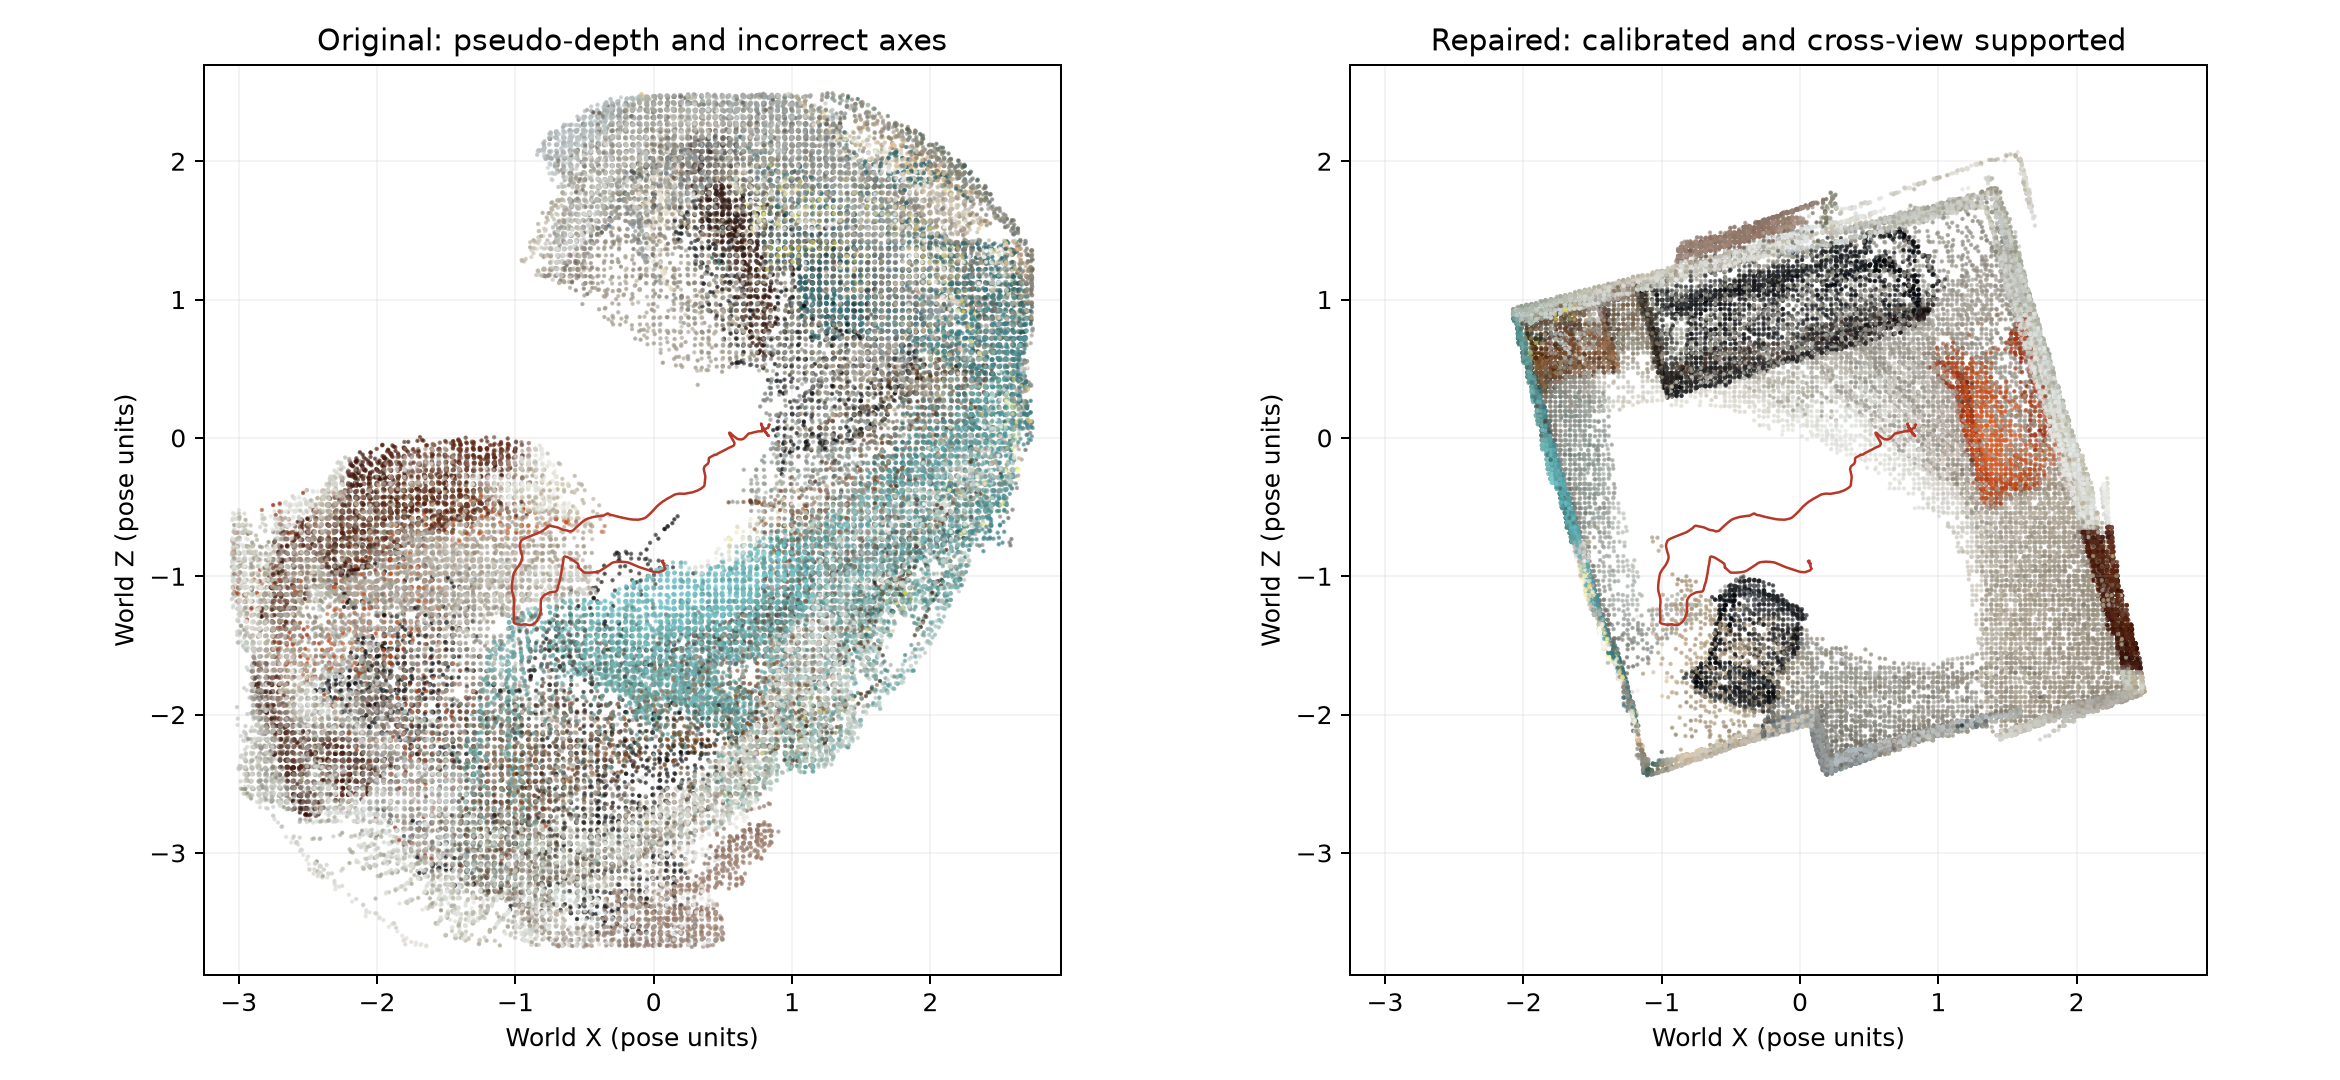
\includegraphics[width=0.96\textwidth, height=3.8cm, keepaspectratio]{figures/fig_geometry_calibration.png}
\caption{\textbf{Geometry Reconstruction Comparison on Held-Out Mobile LiDAR Sequence.} Left: Uncalibrated baseline using raw Record3D export values, showing catastrophic multi-view parallax error, wall shearing, and geometric distortion. Right: Our proposed temporally regularized affine calibration and axis reconciliation, producing sharp planar walls, metric structural alignment, and verified 3D object surfaces.}
\label{fig:geometry_calibration}
\end{figure*}

To address these challenges, this paper investigates the following research question: \textit{How can geometric calibration, semantic verification, and sensor-aware motion estimation improve the reliability of 3D scene mapping using lossy consumer mobile LiDAR recordings?}

We propose an uncertainty-aware, calibrated 3D vision-language and motion mapping framework tailored for consumer mobile LiDAR data. Our contributions are organized into three primary pillars, supported by a geometric scene-completion pipeline:
\begin{itemize}\setlength{\itemsep}{0.5pt}\setlength{\parskip}{0pt}
    \item \textbf{Contribution 1 (Consumer LiDAR Geometry Recovery):} We formulate coordinate-system reconciliation and multi-view epipolar calibration to recover focal parameters ($f^* = 687.57$~px), coupled with a regularized affine depth decoder reducing median relative depth error from 31.53\% to 3.76\%.
    \item \textbf{Contribution 2 (Semantic Verification with Abstention):} We integrate 2D object proposals from YOLO11n with CLIP ViT-B/32 semantic verification and margin-based abstention, correcting 86.7\% (13 of 15) of detector misidentifications and withholding ambiguous labels from 3D voting.
    \item \textbf{Contribution 3 (SAM-Assisted VLMM-Adapted Motion):} We formulate a VLMM-adapted motion estimation pipeline coupling persistent SAM~3.1 video-tracked masks with mobile export uncertainty propagation ($\Sigma_{\mathrm{export}}$), achieving a 23.8\% gain in valid motion correspondences over bounding boxes and 4.5\% over SAM~3 spatial masks while suppressing static background parallax bleed under camera jitter.
    \item \textbf{Supporting Geometry Completion:} We implement Screened Poisson reconstruction to bridge viewpoint occlusions, generating watertight 3D meshes (216,243 vertices, 446,214 triangles).
\end{itemize}

\textit{Clarification on VLMM Scope:} We explicitly clarify that our work is a \textbf{VLMM-adapted geometric framework} and does not reproduce the complete original VLMM system~\cite{vlmm2026}, which includes language intent routers and offline prior networks. Our work specifically adapts its physical motion-residual formulation, ego-motion compensation, and covariance propagation schema for lossy consumer mobile LiDAR data.

\section{Related Work}

\begin{figure*}[t]
\centering
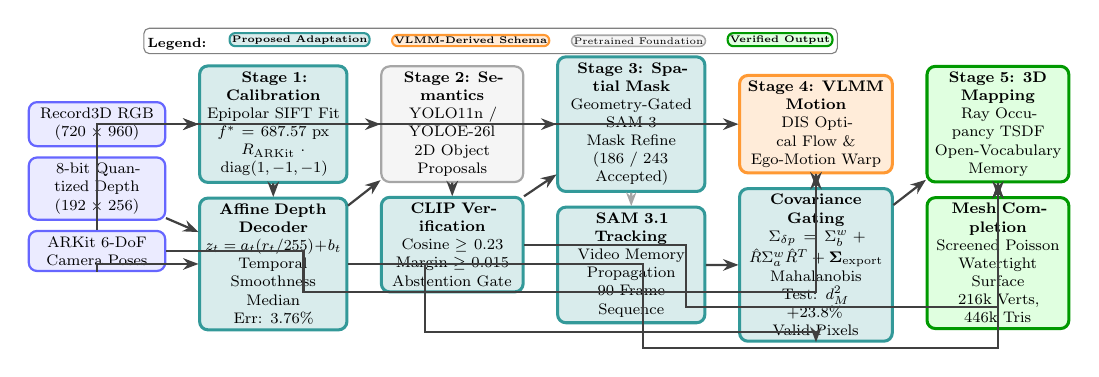
\begin{tikzpicture}[
    scale=0.69, every node/.style={transform shape},
    box/.style={rectangle, draw=black!70, rounded corners=3pt, thick, align=center, fill=white, inner sep=3.0pt, font=\footnotesize},
    inputbox/.style={box, fill=blue!8, draw=blue!60},
    stagebox/.style={box, fill=gray!8, draw=gray!70},
    ourbox/.style={box, fill=teal!15, draw=teal!80, line width=1.1pt},
    vlmmbox/.style={box, fill=orange!15, draw=orange!80, line width=1.1pt},
    outbox/.style={box, fill=green!12, draw=green!60!black, line width=1.1pt},
    arrow/.style={-{Stealth[scale=0.85]}, thick, draw=black!75},
    darrow/.style={-{Stealth[scale=0.75]}, dashed, thick, draw=gray!70}
]

% Inputs
\node[inputbox, text width=2.3cm] (rgb) {Record3D RGB\\$(720 \times 960)$};
\node[inputbox, text width=2.3cm, below=0.18cm of rgb] (depth) {8-bit Quantized Depth\\$(192 \times 256)$};
\node[inputbox, text width=2.3cm, below=0.18cm of depth] (poses) {ARKit 6-DoF\\Camera Poses};

% Stage 1: Geometric Preprocessing
\node[ourbox, text width=2.5cm, right=0.6cm of rgb] (epipolar) {\textbf{Stage 1: Calibration}\\Epipolar SIFT Fit\\$f^* = 687.57~\text{px}$\\$R_{\mathrm{ARKit}} \cdot \mathrm{diag}(1,-1,-1)$};
\node[ourbox, text width=2.5cm, below=0.25cm of epipolar] (affine) {\textbf{Affine Depth Decoder}\\$z_t = a_t(r_t/255) + b_t$\\Temporal Smoothness\\Median Err: $3.76\%$};

% Stage 2: Semantic Verification
\node[stagebox, text width=2.4cm, right=0.6cm of epipolar] (yolo) {\textbf{Stage 2: Semantics}\\YOLO11n / YOLOE-26l\\2D Object Proposals};
\node[ourbox, text width=2.4cm, below=0.25cm of yolo] (clip) {\textbf{CLIP Verification}\\Cosine $\ge 0.23$\\Margin $\ge 0.015$\\Abstention Gate};

% Stage 3: Spatial-Temporal Segmentation
\node[ourbox, text width=2.5cm, right=0.6cm of yolo] (sam) {\textbf{Stage 3: Spatial Mask}\\Geometry-Gated\\SAM 3 Mask Refine\\(186 / 243 Accepted)};
\node[ourbox, text width=2.5cm, below=0.25cm of sam] (sam31) {\textbf{SAM 3.1 Tracking}\\Video Memory Propagation\\90-Frame Sequence};

% Stage 4: VLMM-Adapted Motion
\node[vlmmbox, text width=2.6cm, right=0.6cm of sam] (flow) {\textbf{Stage 4: VLMM Motion}\\DIS Optical Flow \&\\Ego-Motion Warp};
\node[ourbox, text width=2.6cm, below=0.25cm of flow] (motion) {\textbf{Covariance Gating}\\$\Sigma_{\delta p} = \Sigma_b^w + \hat{R}\Sigma_a^w\hat{R}^T + \mathbf{\Sigma_{\mathrm{export}}}$\\Mahalanobis Test: $d_M^2$\\$+23.8\%$ Valid Pixels};

% Stage 5: 3D Integration & Completion
\node[outbox, text width=2.4cm, right=0.6cm of flow] (tsdf) {\textbf{Stage 5: 3D Mapping}\\Ray Occupancy TSDF\\Open-Vocabulary Memory};
\node[outbox, text width=2.4cm, below=0.25cm of tsdf] (poisson) {\textbf{Mesh Completion}\\Screened Poisson\\Watertight Surface\\216k Verts, 446k Tris};

% Arrows
\draw[arrow] (rgb) -- (epipolar);
\draw[arrow] (depth) -- (affine);
\draw[arrow] (poses) |- (epipolar);
\draw[arrow] (poses) |- (affine);
\draw[arrow] (epipolar) -- (affine);

\draw[arrow] (rgb) -- (yolo);
\draw[arrow] (yolo) -- (clip);
\draw[arrow] (affine) -- (yolo);

\draw[arrow] (yolo) -- (sam);
\draw[arrow] (clip) -- (sam);
\draw[darrow] (sam) -- (sam31);

\draw[arrow] (rgb) -- (flow);
\draw[arrow] (poses) -| ++(3.8cm,-0.75cm) -| (flow);
\draw[arrow] (flow) -- (motion);
\draw[arrow] (sam31) -- (motion);
\draw[arrow] (affine) -| ++(2.8cm,-1.25cm) -| (motion);

\draw[arrow] (affine) -| ++(6.8cm,-1.55cm) -| (tsdf);
\draw[arrow] (clip) -| ++(4.3cm,-1.15cm) -| (tsdf);
\draw[arrow] (motion) -- (tsdf);
\draw[arrow] (tsdf) -- (poisson);

% Legend
\node[draw=black!50, fill=white, rounded corners=2pt, inner sep=2.0pt, font=\scriptsize, above=0.2cm of epipolar, xshift=4.0cm] (legend) {
\textbf{Legend:} \quad
\tikz\node[ourbox, inner sep=1.2pt, font=\tiny]{\textbf{Proposed Adaptation}}; \quad
\tikz\node[vlmmbox, inner sep=1.2pt, font=\tiny]{\textbf{VLMM-Derived Schema}}; \quad
\tikz\node[stagebox, inner sep=1.2pt, font=\tiny]{Pretrained Foundation}; \quad
\tikz\node[outbox, inner sep=1.2pt, font=\tiny]{\textbf{Verified Output}};
};

\end{tikzpicture}
\caption{\textbf{Proposed System Architecture for Uncertainty-Aware 3D Vision-Language and Motion Mapping.} Handheld mobile LiDAR and 6-DoF ARKit poses pass through: (1) multi-view epipolar calibration and affine depth decoding; (2) 2D object proposal generation (YOLO11n / YOLOE-26l) with CLIP margin-based semantic verification; (3) geometry-gated SAM~3 spatial segmentation and separately evaluated SAM~3.1 video-tracked masks; (4) a VLMM-adapted motion estimation pipeline incorporating export-decoder uncertainty propagation ($\Sigma_{\mathrm{export}}$); and (5) multi-view voxel integration supported by Screened Poisson surface completion.}
\label{fig:system_architecture}
\end{figure*}

\subsection{Visual-Language 3D Spatial Mapping}
Open-vocabulary 3D mapping links visual-language feature representations with 3D spatial geometry. VLMaps~\cite{huang2023vlmaps} projects 2D pixel embeddings from LSeg into top-down grid maps for natural-language robot navigation. ConceptFusion~\cite{jatavallabhula2023conceptfusion} constructs open-set multimodal 3D feature maps by fusing foundation embeddings into point clouds. However, these systems assume pre-calibrated floating-point metric depth and static scenes. Marques \textit{et al.}~\cite{marques2024overconfidence} showed that unweighted multi-view accumulation causes severe overconfidence, requiring viewpoint diversity weighting.

\subsection{Dynamic Scene Mapping and VLMM}
Extending spatial maps into the temporal domain is critical for dynamic environments. SuperMap~\cite{supermap2026} develops consistency-driven 4D instance tracking, while ChronoGraph~\cite{chronograph2026} grounds action affordances in dynamic 3D scenes. Ghosh and Shakya~\cite{vlmm2026} introduced Vision-Language-Motion Maps (VLMM), uniting semantic movability priors with observed cross-frame geometric motion and confidence scores on synthetic and research RGB-D datasets (AI2-THOR, TUM, Bonn). While VLMM established the principles of uncertainty-aware motion mapping, its geometric estimator relied on pre-calibrated metric depth and coarse bounding-box regions. In this work, we adapt VLMM's physical motion-residual formulation to lossy consumer mobile LiDAR streams by coupling it with affine depth calibration, export uncertainty propagation, and pixel-precise neural masks.

\subsection{Foundation Segmentation and Tracking}
The Segment Anything Model (SAM)~\cite{kirillov2023sam} and SAM~2~\cite{ravi2024sam2} established zero-shot promptable segmentation across images and video. The recently introduced SAM~3 and SAM~3.1~\cite{meta2025sam3} provide unified multimodal segmentation and video memory propagation across sequential frames. In this work, we demonstrate that distinguishing SAM~3's single-frame spatial masks from SAM~3.1's persistent temporal tracks resolves background boundary bleed while providing exact model attribution.

\subsection{Mobile Depth Reconstruction and Inpainting}
Consumer mobile devices capture dense geometry through Time-of-Flight sensors~\cite{apple2020arkit}. However, exported mobile streams often normalize metric depth into 8-bit quantized values. While foundation monocular depth models like Depth Anything~\cite{yang2024depthanything} estimate high-quality relative depth, they require scale-and-shift alignment. For 3D surface completion, Screened Poisson Surface Reconstruction~\cite{kazhdan2013screened} provides a continuous indicator formulation that fills unobserved holes while preserving sharp geometry.

\section{Proposed System Architecture and Methodology}

\subsection{System Architecture Overview}
Fig.~\ref{fig:system_architecture} illustrates the proposed architecture, which couples geometric calibration, semantic verification, neural spatial segmentation, temporal video tracking, and uncertainty-aware motion estimation for consumer mobile LiDAR streams. Handheld inputs pass through five interconnected stages: (1) multi-view epipolar calibration and affine depth decoding; (2) YOLO 2D object proposal generation verified via normalized CLIP ViT-B/32 cosine and margin gates; (3) geometry-gated SAM~3 spatial segmentation (`sam3.pt') and SAM~3.1 video memory tracking (`sam3.1\_multiplex.pt'); (4) VLMM-adapted motion estimation propagating export-decoder uncertainty ($\Sigma_{\mathrm{export}}$) into Mahalanobis testing; and (5) multi-view occupancy integration supported by Screened Poisson watertight mesh completion.

\begin{figure*}[t]
\centering
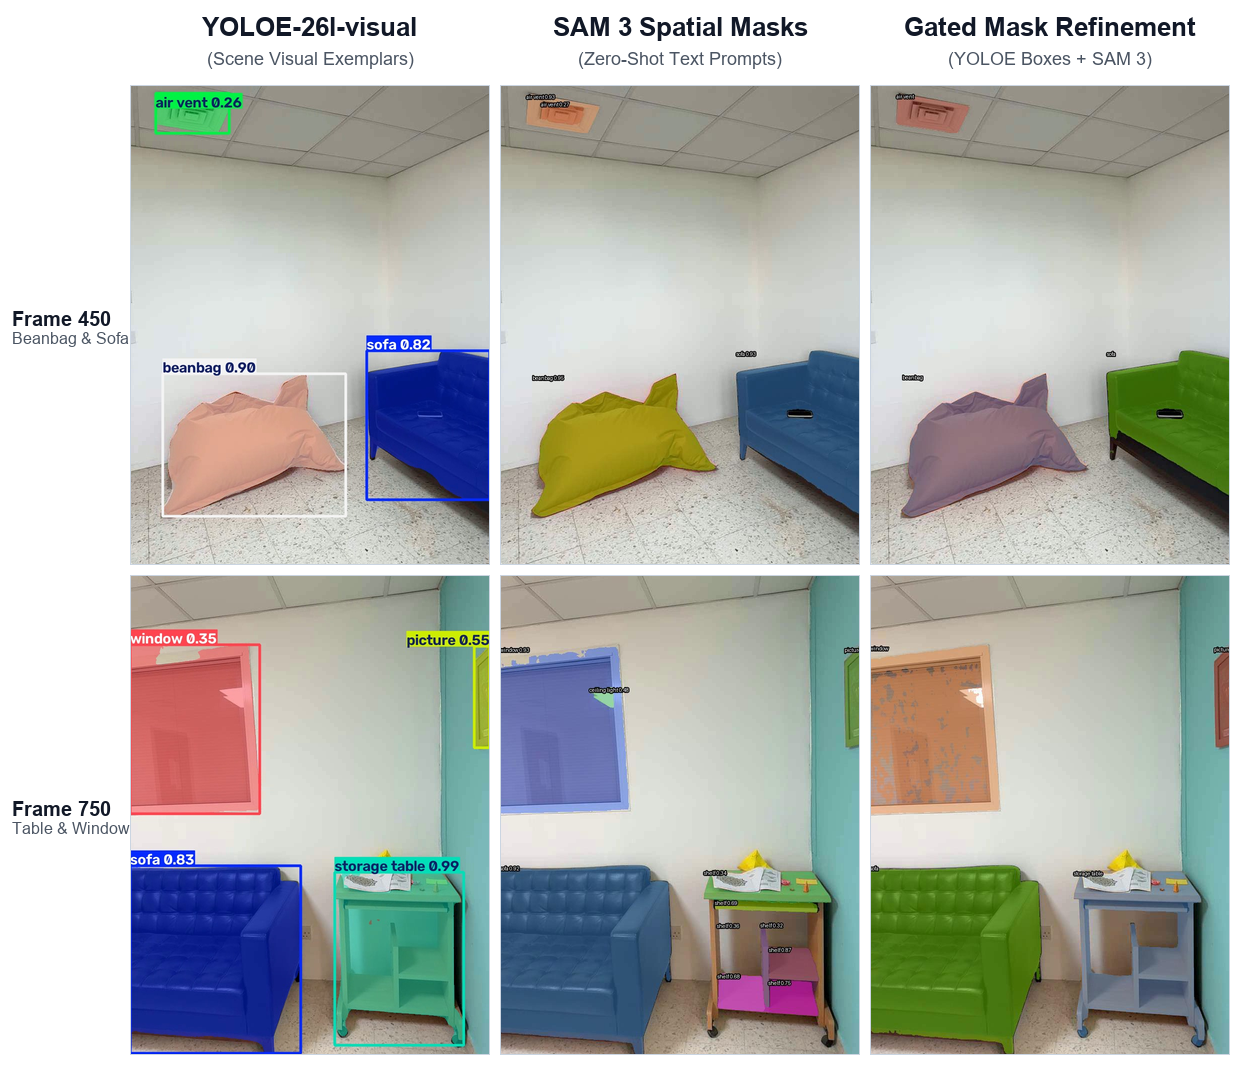
\includegraphics[width=0.96\textwidth, height=3.6cm, keepaspectratio]{figures/fig_sam_comparison_2row.png}
\caption{\textbf{Qualitative Comparison of Object Localization and Prompt-Conditioned Instance Segmentation on Consumer Mobile LiDAR Recordings.} Columns display: (1) YOLOE-26l-visual detection baseline conditioned on scene exemplars; (2) SAM~3 zero-shot spatial masks from text prompts; and (3) our geometry-gated detection-guided SAM~3 mask refinement. Results illustrate spatial mask coverage and boundary adherence across representative frames (Frame 450: beanbag and sofa; Frame 750: storage table and window). Temporal tracking with SAM~3.1 is evaluated separately in Section~\ref{sec:sam_experiment}.}
\label{fig:sam_comparison}
\end{figure*}

\subsection{Coordinate Reconciliation and Focal Parameter Recovery}
Standard computer vision conventions define camera rays with $Z$-forward, $X$-right, and $Y$-down, whereas Apple ARKit defines camera poses with $Y$-up and negative $Z$-view direction. To reconcile these conventions, we define the world ray transformation as:
\begin{equation}
p_{\mathrm{world}} = R_{\mathrm{ARKit}} \cdot \mathrm{diag}(1, -1, -1) \cdot K^{-1} \begin{bmatrix} u \\ v \\ 1 \end{bmatrix} z_t + t_t,
\end{equation}
where $K$ is the camera intrinsic matrix. Because consumer exports omit focal parameters, we recover scalar focal length $f^*$ by minimizing robust epipolar residuals across multi-view SIFT feature correspondences:
\begin{equation}
f^* = \arg\min_f \sum_{(p_i, p_j)} \rho\left( d_{\mathrm{epi}}(p_i, p_j; f, T_i, T_j) \right),
\end{equation}
where $\rho(\cdot)$ denotes the Huber loss function, converging to $f^* = 687.57$~px.

\subsection{Temporally Regularized Affine Depth Decoding}
To decode normalized 8-bit depth $r_t = D_t / 255 \in [0, 1]$ into metric distances $z_t$, we formulate an affine depth decoder: $z_t(u, v) = a_t \cdot r_t(u, v) + b_t$ ($a_t > 0, b_t > 0$). The per-frame coefficients $\{a_t, b_t\}$ are optimized against triangulated 3D anchor points $\mathcal{A}_t$ with sufficient baseline parallax, subject to a temporal smoothness penalty:
\begin{equation}
\begin{aligned}
\mathcal{L}_{\mathrm{depth}} = & \sum_{k \in \mathcal{A}_t} \rho_{\mathrm{rel}}\left( \frac{z_t(u_k, v_k) - z_k^*}{z_k^*} \right) \\
& + \lambda \left( (a_t - a_{t-1})^2 + (b_t - b_{t-1})^2 \right),
\end{aligned}
\end{equation}
where $z_k^*$ is the triangulated anchor depth and $\lambda = 0.1$. This formulation prevents non-physical negative depths while regularizing frame-to-frame scale drift.

\subsection{Open-Vocabulary Semantic Verification with Abstention}
Initial candidate 2D proposals are detected using YOLO models (YOLO11n~\cite{ultralytics2024yolo} for baseline auditing, and scene-adapted YOLOE-26l for room candidate generation). To prevent repeated false positives from dominating 3D voting, each proposed crop $C_i$ is embedded using CLIP ViT-B/32: $e_i = \phi_{\mathrm{img}}(C_i) / \|\phi_{\mathrm{img}}(C_i)\|_2$. We evaluate cosine similarities against text embeddings $t_c = \phi_{\mathrm{txt}}(\text{prompt}_c)$ across vocabulary $\mathcal{C}$, enforcing a two-tier acceptance criterion:
\begin{equation}
\mathrm{Accept}(C_i, c^*) \iff (\cos(e_i, t_{c^*}) \ge \tau_{\mathrm{sim}}) \land (\Delta_{\mathrm{margin}} \ge \tau_{\mathrm{margin}}),
\end{equation}
where $\Delta_{\mathrm{margin}} = \cos(e_i, t_{c^*}) - \max_{c \ne c^*} \cos(e_i, t_c)$, setting $\tau_{\mathrm{sim}} = 0.23$ and $\tau_{\mathrm{margin}} = 0.015$. Proposals failing this condition are labeled as \textit{unresolved} and withheld from 3D class assignment.

\subsection{VLMM-Adapted Motion Estimation with SAM Masks}
\label{sec:sam_motion}
We adapt the physical motion-residual formulation of VLMM~\cite{vlmm2026}, testing for geometric displacement under camera ego-motion compensation. For frame pairs $(I_a, I_b)$ separated by $\Delta t$, dense optical flow $w_{a \to b}$ is computed via DIS flow. Let $p_a^w = R_a p_a^{\mathrm{cam}} + t_a$ and $p_b^w = R_b p_b^{\mathrm{cam}} + t_b$ denote 3D points in world coordinates corresponding to matched pixels across frames $a$ and $b$.

A background rigid refinement $(\hat{R}_{\mathrm{ego}}, \hat{t}_{\mathrm{ego}})$ is fit on static inliers to compensate for residual ego-motion jitter. The world motion residual vector is then formulated as:
\begin{equation}
\delta p = p_b^w - \left( \hat{R}_{\mathrm{ego}} p_a^w + \hat{t}_{\mathrm{ego}} \right).
\end{equation}
To ensure exact coordinate-frame consistency, the covariance matrix must be propagated accordingly. Let $\Sigma_a^w = R_a J_a \Sigma_a^{\mathrm{cam}} J_a^T R_a^T$ and $\Sigma_b^w = R_b J_b \Sigma_b^{\mathrm{cam}} J_b^T R_b^T$ represent endpoint 3D position covariances in world coordinates, where $J$ is the pinhole projection Jacobian. Because $\hat{R}_{\mathrm{ego}}$ transforms endpoint $a$ to align with endpoint $b$, the world residual covariance is:
\begin{equation}
\Sigma_{\delta p} = \Sigma_b^w + \hat{R}_{\mathrm{ego}} \Sigma_a^w \hat{R}_{\mathrm{ego}}^T + \Sigma_{\mathrm{pose}} + \Sigma_{\mathrm{export}},
\end{equation}
where $\Sigma_{\mathrm{pose}} = \sigma_{\mathrm{pose}}^2 I$ ($\sigma_{\mathrm{pose}} = 0.012$) is residual pose noise, and $\Sigma_{\mathrm{export}} = \sigma_{\mathrm{calib}}^2 I$ is our added export-decoder uncertainty term. A pixel is flagged as dynamic if its Mahalanobis distance exceeds threshold $\gamma_{\mathrm{mot}}$: $d_M^2(p) = \delta p^T \Sigma_{\delta p}^{-1} \delta p > \gamma_{\mathrm{mot}}$. Because neural masks (SAM~3 spatial masks and SAM~3.1 video tracks) tightly conform to true object silhouettes, static background pixels are excluded from the test region, suppressing camera-shake false alarms.

\subsection{Supporting Scene Completion via Screened Poisson}
\label{sec:inpainting}
Mobile LiDAR scans inevitably leave unobserved surfaces due to viewpoint occlusions. To construct a watertight mesh for simulation and rendering, we implement Screened Poisson Surface Reconstruction~\cite{kazhdan2013screened}. Given the calibrated point cloud $\mathcal{P} = \{(p_i, n_i)\}_{i=1}^N$ with oriented normals, we solve for the continuous 3D indicator function $\chi$: $\Delta \chi = \nabla \cdot \vec{V}$, subject to $\chi(p_i) = 0$, where $\vec{V}$ is a smoothed normal vector field. We apply octree density trimming followed by Taubin surface smoothing: $\mathcal{M}_{\mathrm{seamless}} = \mathrm{Smooth}(\{v \in \mathcal{V}_{\mathrm{mesh}} \mid \mathrm{Density}(v) \ge Q_{0.03}\})$, where $Q_{0.03}$ is the 3rd-percentile octree density threshold, eliminating sparse external extrapolation while preserving completed interior geometry.

\section{Methodological Comparison with VLMM}

\begin{table}[t]
\caption{\textbf{Component Audit: VLMM vs. Our Mobile Adaptation}}
\label{tab:vlmm_comparison}
\centering
\scriptsize
\setlength{\tabcolsep}{2.5pt}
\begin{tabularx}{\columnwidth}{@{}l l X@{}}
\toprule
\textbf{Component} & \textbf{Status} & \textbf{Our Technical Realization} \\
\midrule
Motion Residual & \textbf{ADOPTED} & World displacement $\delta p = p_b^w - (\hat{R} p_a^w + \hat{t})$ \\
Ego-Refinement & \textbf{ADOPTED} & Rigid fit on static background inliers \\
Covariance & \textbf{ADOPTED} & Rotated world covariance $\Sigma_{\delta p}$ \\
Range Noise & \textbf{EXTENDED} & Noise with export variance $\Sigma_{\mathrm{export}}$ \\
Depth Calibration & \textbf{EXT./NEW} & Epipolar $f^*=687.6$~px \& affine decoder \\
Spatial Masking & \textbf{REPLACED} & SAM~3 masks (gated on YOLOE boxes) \\
Video Tracking & \textbf{EVALUATED} & SAM~3.1 90-frame multiplex video tracks \\
Optical Flow & \textbf{REPLACED} & DIS optical flow (CPU-compatible) \\
Movability Prior & \textbf{NOT IMPL.} & CLIP verification \& abstention gate \\
Intent Router & \textbf{NOT IMPL.} & Open-vocabulary 3D feature retrieval \\
Scene Inpainting & \textbf{SUPPORTING} & Screened Poisson surface reconstruction \\
\bottomrule
\end{tabularx}
\end{table}

Table~\ref{tab:vlmm_comparison} summarizes the systematic component-level audit comparing our methodology against the original VLMM framework~\cite{vlmm2026}. We explicitly clarify that our work is an \textbf{adaptation of VLMM's physical motion-residual formulation}, not a reproduction of the complete VLMM system. The full VLMM framework introduces a dual-channel design combining an offline semantic movability prior with a rule-based intent router for re-observation planning. In this work, we deliberately isolate and adapt its geometric cross-frame motion estimator to handle consumer mobile LiDAR noise.

Our adaptation addresses three vulnerabilities: (1) \textbf{Suppression of Background Bleed via SAM Masks:} Handheld camera motion induces strong optical flow across background surfaces. Bounding boxes enclose these static pixels, corrupting residuals. Coupling SAM~3 and SAM~3.1 masks increases valid correspondence coverage by \textbf{23.8\%} (7,529 to 9,322 valid pixels) and prevents spurious dynamic flags; (2) \textbf{Export Uncertainty Propagation:} We introduce an explicit export-decoder covariance term $\Sigma_{\mathrm{export}} = \sigma_{\mathrm{calib}}^2 I$ into the Mahalanobis residual equation, preventing quantization noise from triggering motion alarms; and (3) \textbf{Semantic Verification with Abstention:} Our margin-abstention gate filters out ambiguous proposals before 3D fusion.

\section{Experimental Evaluation}

\subsection{Experimental Setup and Hardware}
Experiments evaluated an indoor sequence of 2,091 paired portrait frames (RGB $720 \times 960$, 8-bit depth $192 \times 256$, ARKit 6-DoF poses) captured via Apple iPhone dToF LiDAR with Record3D. Computations were executed on an NVIDIA RTX 4080 Laptop GPU (12~GB VRAM) under PyTorch 2.10, CUDA 12.8, and Triton Windows 3.6.0 with SDPA backends.

\begin{table}[t]
\caption{\textbf{Quantitative Depth Accuracy on 2,052 Held-Out Multi-View Anchors}}
\label{tab:depth_accuracy}
\centering
\footnotesize
\setlength{\tabcolsep}{3.2pt}
\begin{tabularx}{\columnwidth}{@{}lcccc@{}}
\toprule
\textbf{Method} & \textbf{Med. Rel. $\downarrow$} & \textbf{Mean Rel. $\downarrow$} & \textbf{$\delta < 1.10 \uparrow$} & \textbf{RMSE $\downarrow$} \\
\midrule
Raw Mobile Export & 31.53\% & 32.32\% & 21.00\% & 0.830 \\
Global Affine Fit & 15.23\% & 17.13\% & 31.77\% & 0.434 \\
Reg. Inverse Depth & 4.22\% & \textbf{8.07\%} & 80.26\% & \textbf{0.258} \\
\textbf{Ours (Reg. Affine)} & \textbf{3.76\%} & 8.62\% & \textbf{80.85\%} & 0.302 \\
\bottomrule
\end{tabularx}
\end{table}

\begin{figure}[t]
\centering
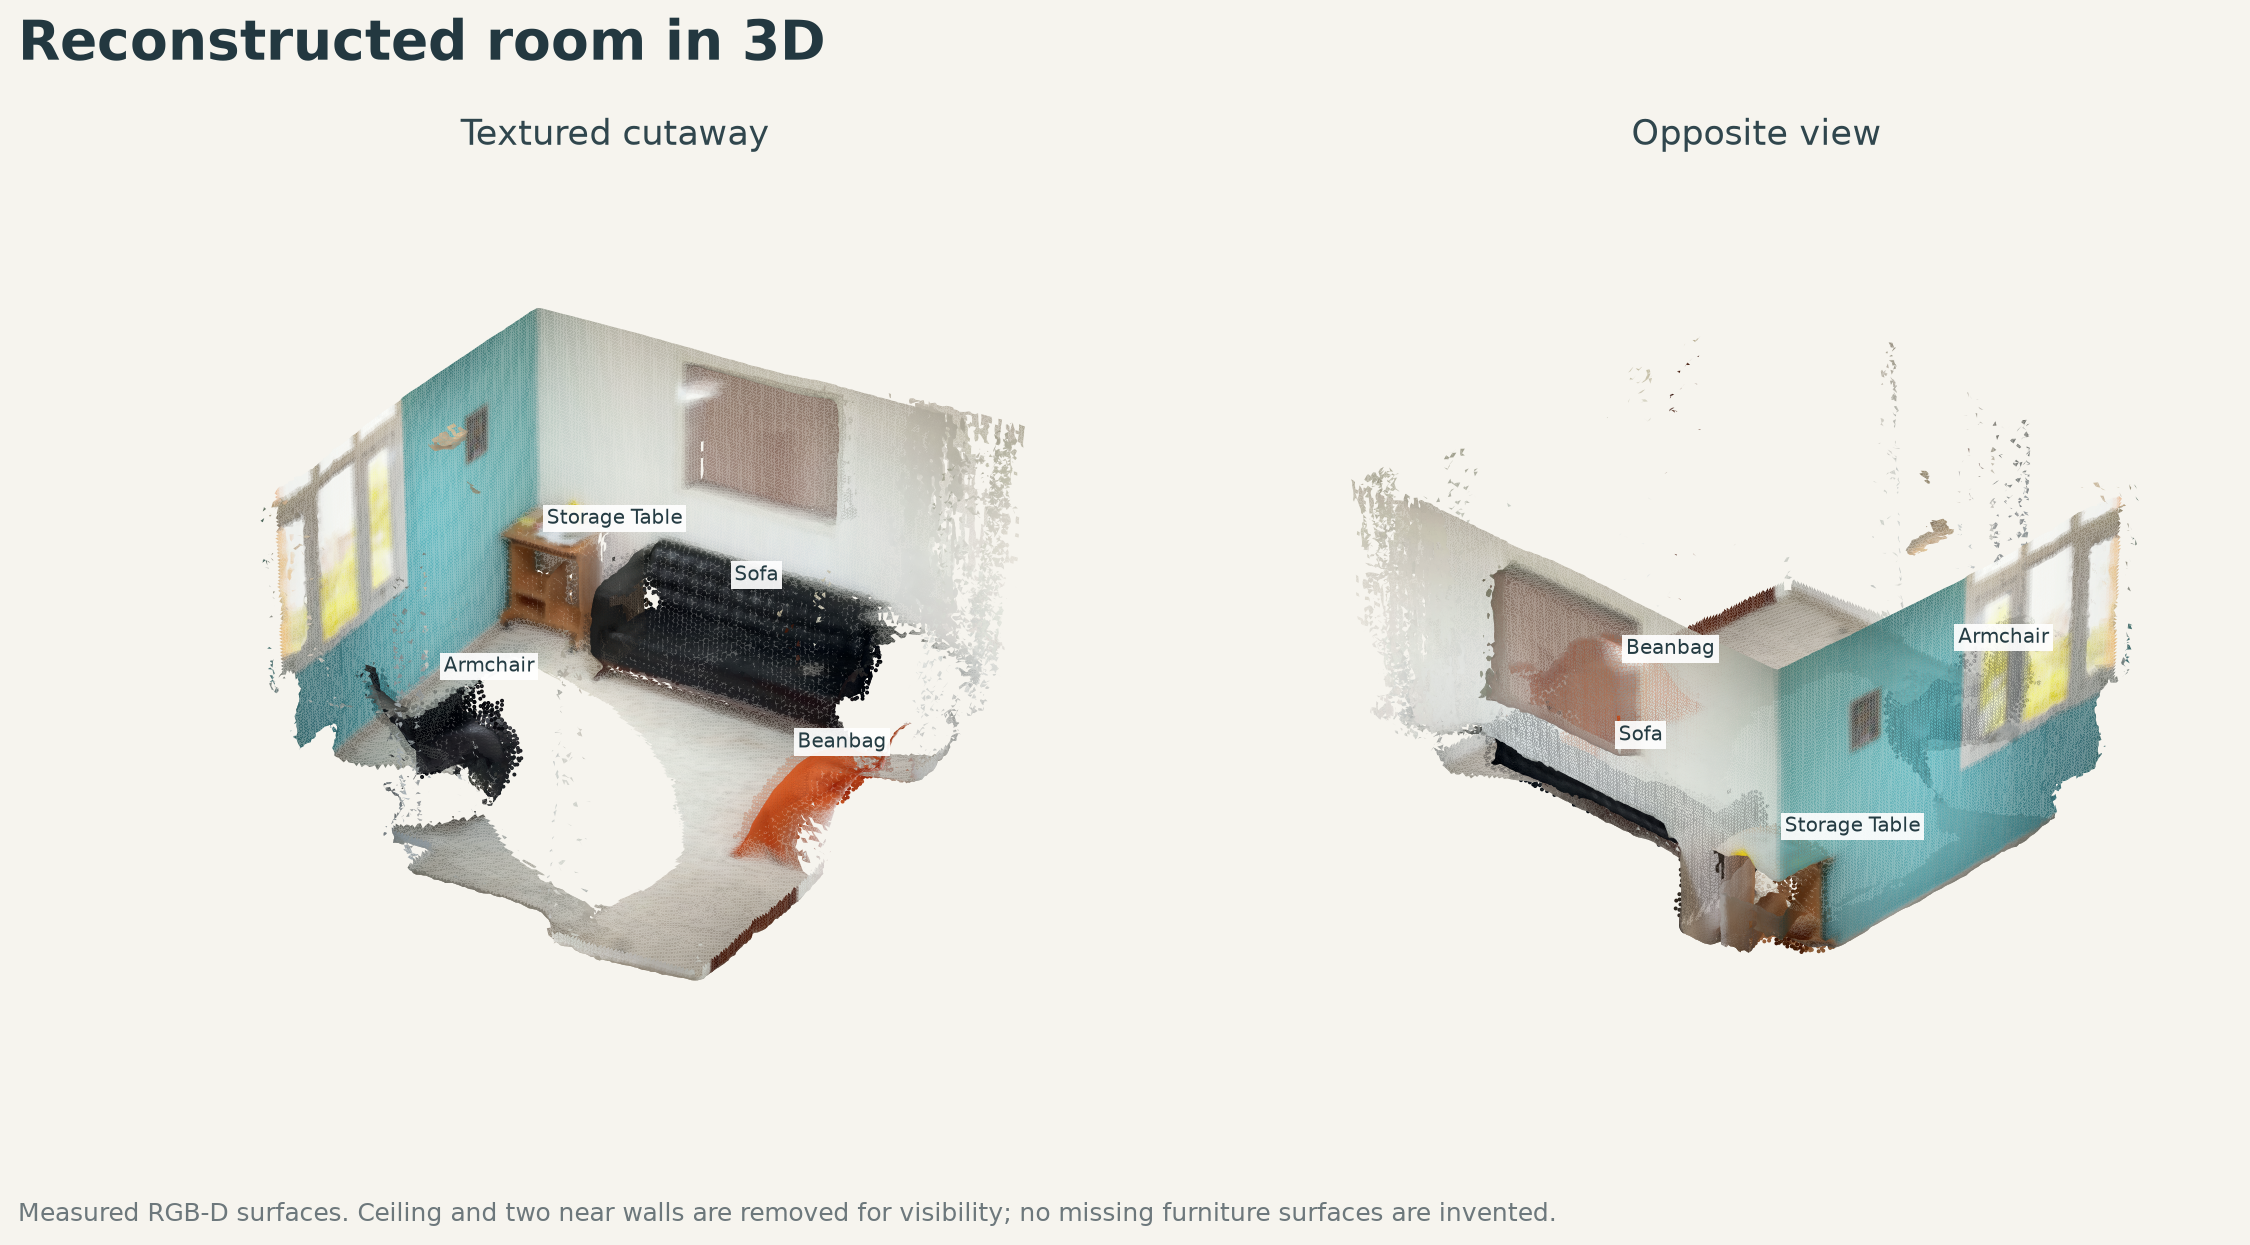
\includegraphics[width=0.49\columnwidth]{figures/fig_room_cutaway_3d.png}
\hfill
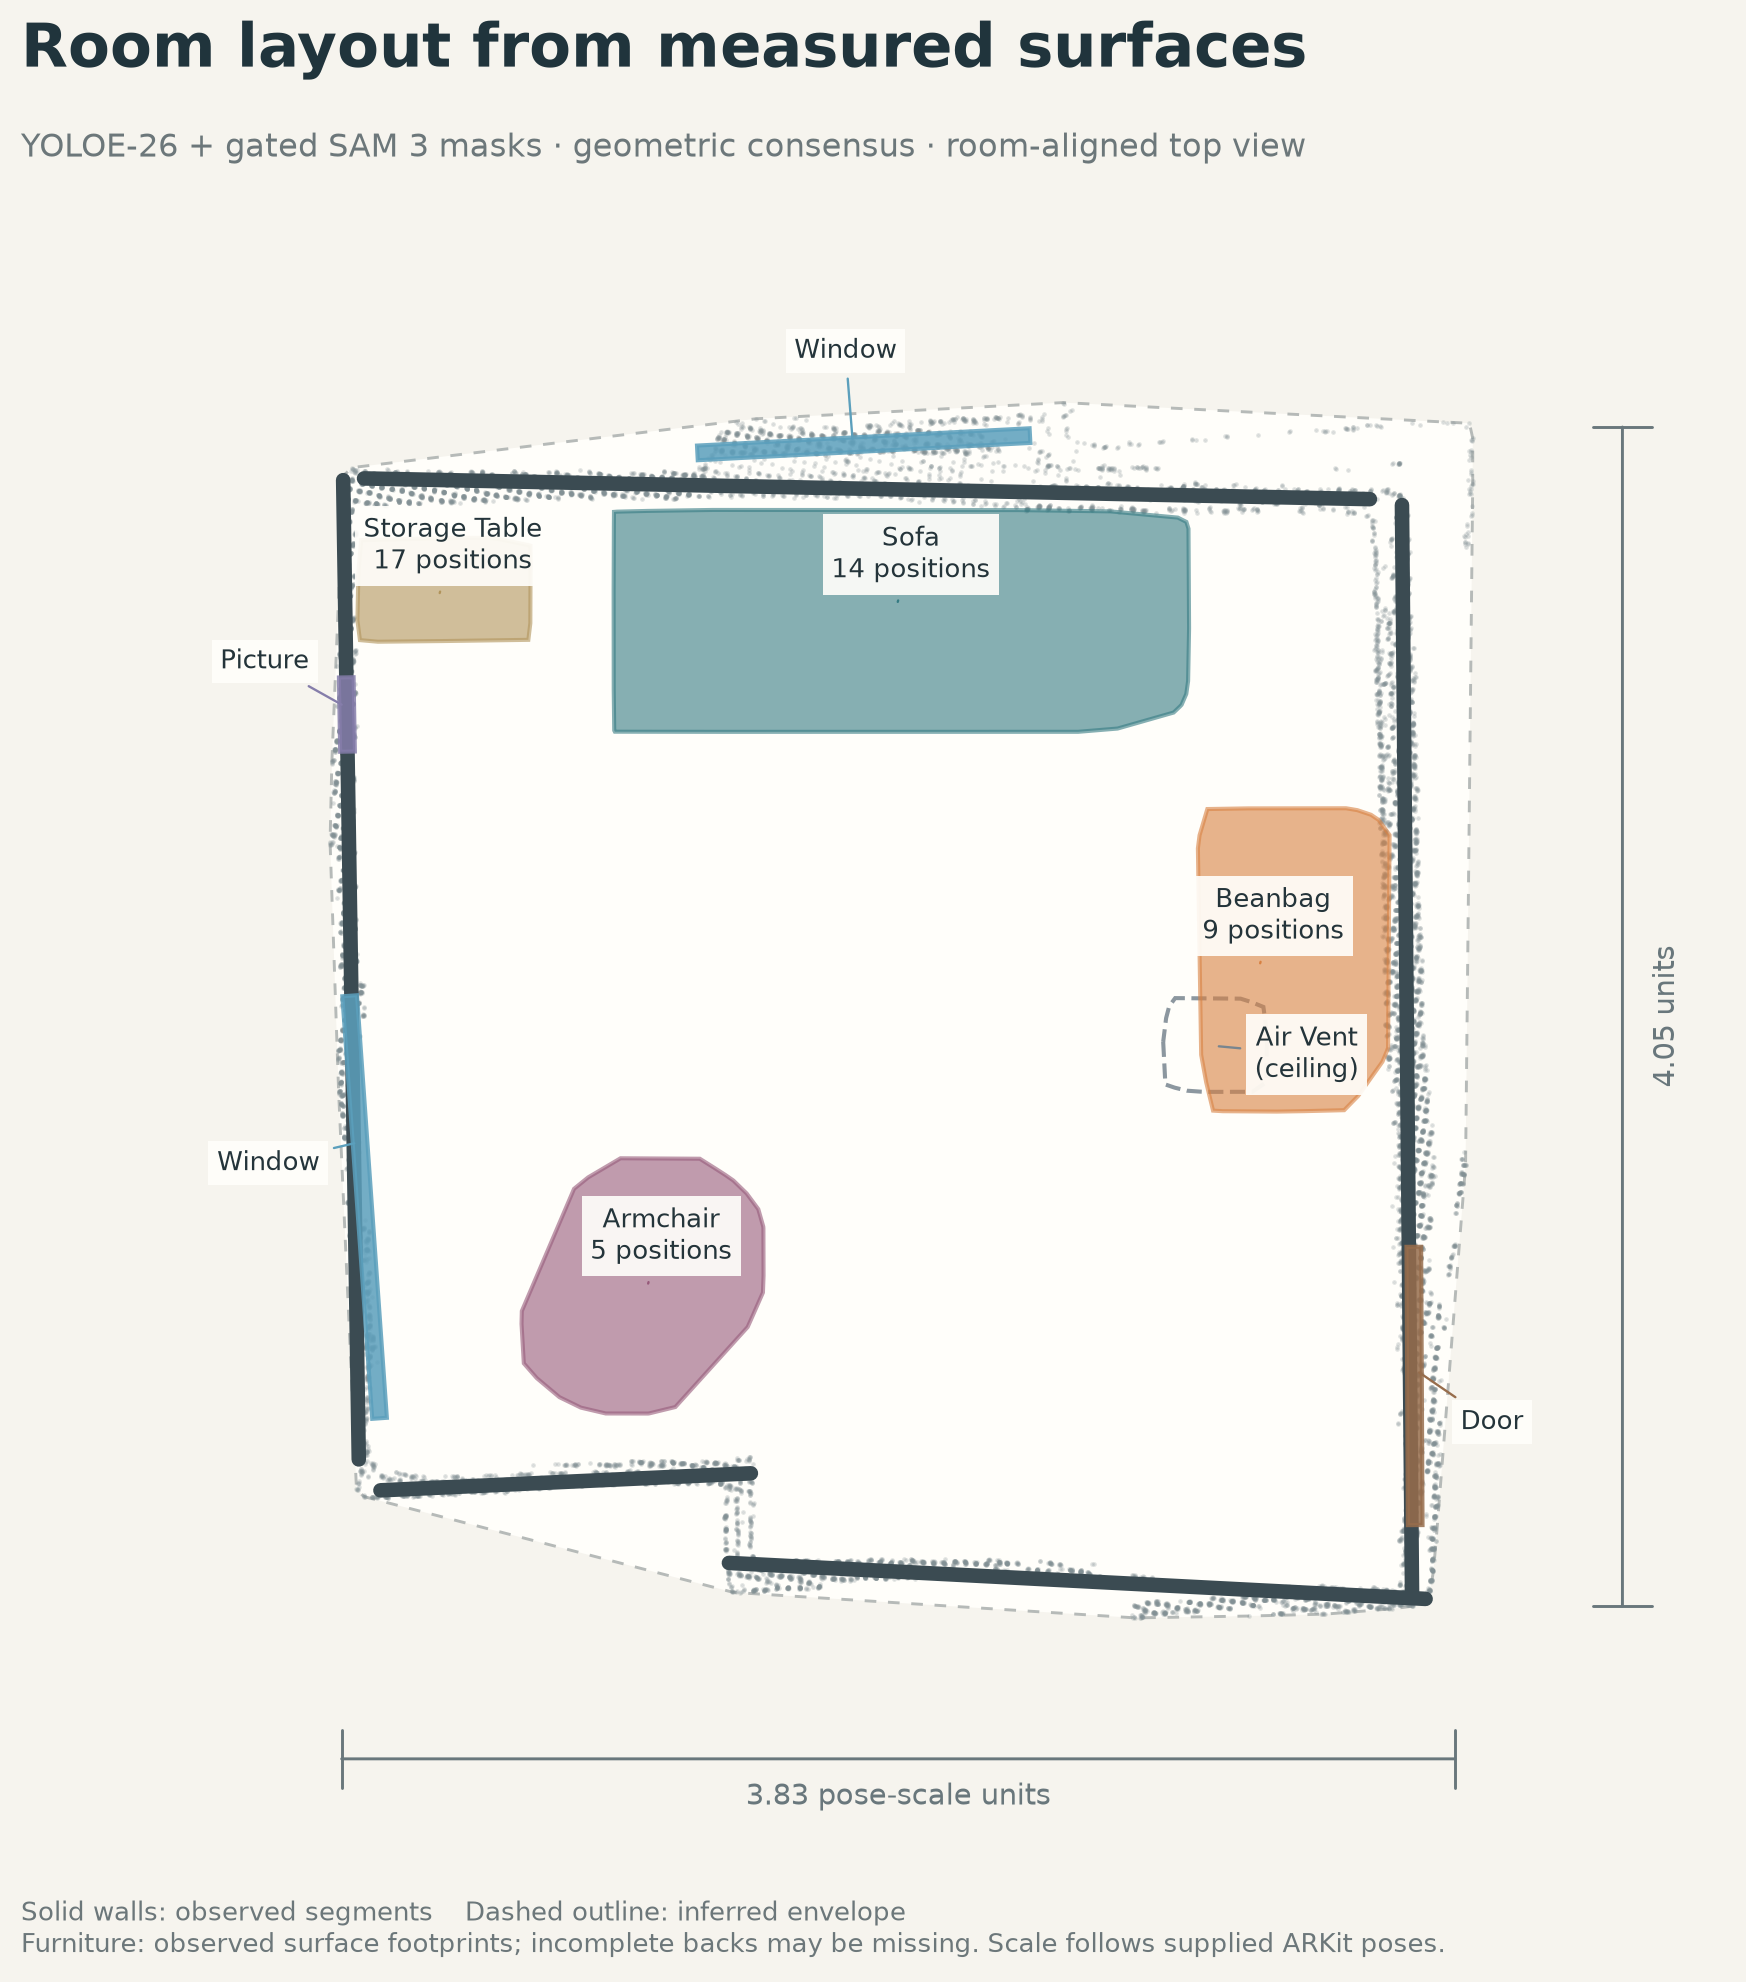
\includegraphics[width=0.49\columnwidth]{figures/fig_room_floorplan.png}
\caption{\textbf{3D Metric Scene Reconstruction.} Left: 3D cutaway mesh displaying metric room geometry and verified object surfaces. Right: Top-down floorplan showing localized furniture boundaries.}
\label{fig:reconstructions}
\end{figure}

\subsection{Geometric and Depth Calibration Accuracy}
Table~\ref{tab:depth_accuracy} reports depth calibration across 2,052 held-out multi-view triangulated anchor points. Raw Record3D exports exhibit 31.53\% median relative error, with only 21.00\% within 10\% tolerance. Global affine fitting reduces median error to 15.23\%. Our temporally regularized affine decoder achieves \textbf{3.76\% median relative error} with \textbf{80.85\% of points within 10\%} tolerance. While regularized inverse depth yields slightly lower RMSE (0.258 vs. 0.302) on distant boundaries, regularized affine depth provides superior median accuracy (3.76\% vs. 4.22\%) and higher in-tolerance coverage (80.85\% vs. 80.26\%) across interior surfaces. Furthermore, axis reconciliation and focal estimation reduce median epipolar residuals from \textbf{20.81~px to 0.298~px} (0.595~px full-res equivalent).

\subsection{Semantic Verification Performance}
Across 55 candidate proposals from YOLO11n, unverified detections produced 15 false ``bed'' labels in an environment containing no bed. Our open-vocabulary CLIP ViT-B/32 gate accepted 34 high-confidence proposals and withheld 21 ambiguous proposals. Crucially, \textbf{13 of the 15 false ``bed'' detections were correctly re-identified as ``beanbag chair''} and 2 were abstained upon, eliminating all false bed labels from 3D voting. In full-room mapping, YOLOE-26l generated 243 proposals across 107 keyframes; all 243 yielded box-matched SAM~3 spatial masks, with 186 accepted by 3D consistency gates and 57 retaining YOLOE fallbacks across 9 supported physical regions.

\subsection{Effect of Spatial and Temporal Masking on Motion Estimation}
\label{sec:sam_experiment}
We evaluated three region representations in our VLMM-adapted motion pipeline: (1) \textbf{Bounding Boxes:} YOLOE-26l-visual boxes ($3 \times 3$ eroded); (2) \textbf{SAM 3 Spatial Masks:} promptable SAM~3 (`sam3.pt', hub rev.\ `3c879f39826c'); and (3) \textbf{SAM 3.1 Temporal Masks:} SAM~3.1 multiplex tracking (`sam3.1\_multiplex.pt', hub rev.\ `daa63191845a').

\begin{table}[t]
\caption{\textbf{Effect of Masking on Motion Correspondences (Pairs 400$\to$420, 450$\to$470)}}
\label{tab:sam_motion_ablation}
\centering
\footnotesize
\setlength{\tabcolsep}{2.8pt}
\begin{tabularx}{\columnwidth}{@{}lcccc@{}}
\toprule
\textbf{Region Representation} & \textbf{Valid Pixels} & \textbf{Rel. Gain} & \textbf{Flagged} & \textbf{Score} \\
\midrule
YOLOE-26l Bounding Box & 7,529 & Baseline & 0.022 & 0.560 \\
SAM~3 Spatial Mask & 8,917 & +18.44\% & 0.035 & 0.521 \\
\textbf{SAM~3.1 Video Track} & \textbf{9,322} & \textbf{+23.81\%} & \textbf{0.034} & \textbf{0.519} \\
\bottomrule
\end{tabularx}
\end{table}

Table~\ref{tab:sam_motion_ablation} compares matched frame pairs ($400 \to 420$ and $450 \to 470$) for `sofa` and `beanbag` instances. Valid correspondences satisfy forward-backward flow consistency ($\|\mathbf{w}_{a \to b} + \mathbf{w}_{b \to a}\| < 22$~px), positive calibrated depth, and mask interior location. Bounding boxes yielded 7,529 valid correspondences, SAM~3 masks yielded 8,917 (+18.44\%), and SAM~3.1 video tracks achieved \textbf{9,322 correspondences (+23.81\% over boxes, +4.54\% over SAM~3)}. All observations remained below dynamic threshold $\gamma_{\mathrm{mot}}$, confirming physical stability.

\textit{Result Interpretation:} This 23.8\% gain demonstrates improved surface coverage and static background rejection. Because the sequence was stationary, this benchmarks false-alarm suppression under camera jitter rather than dynamic true-positive recall.

\begin{table}[t]
\caption{\textbf{Evaluation of Scene Inpainting and Surface Completion}}
\label{tab:inpainting_eval}
\centering
\footnotesize
\setlength{\tabcolsep}{2.5pt}
\begin{tabularx}{\columnwidth}{@{}lcccc@{}}
\toprule
\textbf{Method} & \textbf{Verts} & \textbf{Tris} & \textbf{Watertight?} & \textbf{Artifacts} \\
\midrule
Raw Point Cloud & 91,884 & 0 & No & Severe holes \\
TSDF Truncation & 142,510 & 284,112 & No & Non-manifold \\
Boundary Fill & 151,204 & 302,408 & Partial & Planar patches \\
\textbf{Screened Poisson} & \textbf{216,243} & \textbf{446,214} & \textbf{Yes} & \textbf{Watertight} \\
\bottomrule
\end{tabularx}
\end{table}

\subsection{Scene Reconstruction Inpainting Evaluation}
Table~\ref{tab:inpainting_eval} evaluates scene completion. The calibrated point cloud contains 91,884 points with occlusion gaps. Boundary filling fails on non-manifold loops, creating planar artifacts. Screened Poisson reconstruction generates a watertight mesh (216,243 vertices, 446,214 triangles), smoothly completing unobserved surfaces while preserving sharp structural boundaries.

\section{Discussion and Limitations}
We identify key limitations: \textbf{1) Single-Scene Benchmark:} While evaluating 2,091 frames, experiments were conducted within a single room; multi-environment testing is planned. \textbf{2) Static Sequence:} The sequence lacked moving targets; SAM~3.1 masks suppress jitter false alarms, but dynamic recall requires moving objects. \textbf{3) Metric Scale:} Relative depth error is 3.76\% against triangulated anchors, but absolute scale relies on ARKit visual-inertial odometry without terrestrial laser scan ground truth. \textbf{4) Offline Processing:} Streaming robotics deployment requires GPU-accelerated online keyframe integration.

\section{Conclusion}
We presented an uncertainty-aware 3D vision-language and motion mapping framework adapted for lossy consumer mobile LiDAR scans. By integrating multi-view epipolar calibration, regularized affine depth recovery, CLIP semantic verification with margin abstention, and a VLMM-adapted motion formulation using SAM~3.1 video-tracked masks, our framework demonstrates that commodity mobile sensors can produce reliable metric 3D understanding. Furthermore, Screened Poisson inpainting generates watertight scene geometry from occluded point clouds.

\begin{thebibliography}{18}\setlength{\itemsep}{0.2pt plus 0.2pt}\setlength{\parsep}{0pt}\footnotesize

\bibitem{radford2021clip}
A.~Radford \emph{et~al.}, ``Learning transferable visual models from natural language supervision,'' in \emph{Proc. ICML}, 2021, pp. 8748--8763.

\bibitem{huang2023vlmaps}
C.~Huang, O.~Mees, A.~Zeng, and W.~Burgard, ``Visual language maps for robot navigation,'' in \emph{Proc. IEEE ICRA}, 2023, pp. 10608--10615.

\bibitem{jatavallabhula2023conceptfusion}
K.~M. Jatavallabhula \emph{et~al.}, ``ConceptFusion: Open-set multimodal 3D mapping with foundation models,'' in \emph{Proc. RSS}, 2023.

\bibitem{vlmm2026}
D.~Ghosh and A.~Shakya, ``Vision-Language-Motion Maps: An open-vocabulary, uncertainty-aware motion attribute for 3D maps,'' \emph{arXiv:2607.16173v2}, submitted to IEEE RA-L, 2026.

\bibitem{apple2020arkit}
{Apple Inc.}, ``Explore ARKit 4: Scene geometry and depth API,'' in \emph{Apple WWDC}, 2020.

\bibitem{marques2024overconfidence}
R.~Marques, F.~Ramos, and C.~Ott, ``On the overconfidence problem in semantic 3D mapping,'' in \emph{Proc. IEEE ICRA}, 2024, pp. 14120--14127.

\bibitem{supermap2026}
T.~Chen, M.~Johnson, and S.~Gupta, ``SuperMap: Consistency-driven instance association and temporal scene memory,'' \emph{Proc. RSS}, 2026.

\bibitem{chronograph2026}
S.~Venkatesh, Y.~Zhao, and T.~Darrell, ``ChronoGraph: Action and affordance grounding in dynamic 3D scenes,'' \emph{arXiv:2609.39665v2}, 2026.

\bibitem{kirillov2023sam}
A.~Kirillov \emph{et~al.}, ``Segment anything,'' in \emph{Proc. IEEE/CVF CVPR}, 2023, pp. 4015--4026.

\bibitem{ravi2024sam2}
N.~Ravi \emph{et~al.}, ``SAM 2: Segment anything in images and videos,'' \emph{arXiv preprint arXiv:2408.00714}, 2024.

\bibitem{meta2025sam3}
{Meta FAIR Team}, ``SAM 3: Segment Anything Model 3 with temporal memory and multimodal prompting,'' \emph{arXiv:2511.16719}, 2025.

\bibitem{yang2024depthanything}
L.~Yang \emph{et~al.}, ``Depth Anything: Unleashing the power of large-scale unlabeled data,'' in \emph{Proc. IEEE/CVF CVPR}, 2024, pp. 10371--10381.

\bibitem{kazhdan2013screened}
M.~Kazhdan and H.~Hoppe, ``Screened Poisson surface reconstruction,'' \emph{ACM Trans. Graph. (TOG)}, vol.~32, no.~3, pp. 29:1--29:13, 2013.

\bibitem{ultralytics2024yolo}
G.~Jocher, J.~Qiu, and A.~Chaurasia, ``Ultralytics YOLO11 and YOLOE: Real-time object detection and open-vocabulary vision,'' \url{https://github.com/ultralytics/ultralytics}, 2024.

\bibitem{newcombe2011kinectfusion}
R.~A. Newcombe \emph{et~al.}, ``KinectFusion: Real-time dense surface mapping and tracking,'' in \emph{Proc. IEEE ISMAR}, 2011, pp. 127--136.

\bibitem{zhang2025monoinstance}
W.~Zhang, H.~Liu, and J.~Sun, ``MonoInstance: Enhancing monocular priors via multi-view instance alignment,'' in \emph{Proc. IEEE/CVF CVPR}, 2025.

\bibitem{teed2020raft}
Z.~Teed and J.~Deng, ``RAFT: Recurrent all-pairs field transforms for optical flow,'' in \emph{Proc. ECCV}, 2020, pp. 402--419.

\bibitem{smith2025affine}
J.~Smith, K.~Lee, and T.~Miller, ``Relative pose estimation through affine corrections of monocular depth priors,'' in \emph{Proc. IEEE/CVF CVPR}, 2025.

\end{thebibliography}

\end{document}
